\documentclass{article}
\usepackage[T1]{fontenc}
\usepackage[utf8]{inputenc}
\usepackage[a4paper, total={6in, 11in}]{geometry}
\usepackage{algorithm}
\usepackage{amsfonts}
\usepackage{algpseudocode}
\usepackage{float}
\usepackage{graphicx}
\usepackage{subcaption}

\def\v{0.47}

\title{%
	Obliczenia naukowe \\
	\large Lista 4}
\author{Szymon Janiak}
\begin{document}
\maketitle

\section*{Zadanie 1}
\subsection*{Opis problemu}
	Napisać funkcję obliczającą ilorazy różnicowe dla podanych węzłów oraz wartości danej funkcji w tych węzłach.
\subsection*{Dane wejściowe}\label{1.in-data}
	\begin{itemize}
		\item \texttt{x} — wektor długości $n+1$ zawierający węzły $x_0,\dots,x_n$
		\item \texttt{f} — wektor długości $n+1$ zawierający wartości interpolowanej funkcji w węzłach $f(x_0), \dots, f(x_n)$
	\end{itemize}
\subsection*{Dane wyjściowe}
	\begin{itemize}
	    \item \texttt{fx} — wektor długości $n+1$ zawierający obliczone ilorazy różnicowe
	\end{itemize}
\subsection*{Opis użytego algorytmu}

\section*{Zadanie 2}
\subsection*{Opis problemu}
	Napisać funkcję obliczającą wartość wielomianu interpolacyjnego stopnia $n$ w postaci Newtona $N_n(x)$ w punkcie $x = t$ za pomocą algorytmu uogólnionego Hornera w czasie $O(n)$.
\subsection*{Dane wejściowe}
	\begin{itemize}
	    \item \texttt{x} — wektor długości $n+1$ zawierający węzły $x_0,\dots,x_n$
	    \item \texttt{fx} — wektor długości $n+1$ zawierający ilorazy różnicowe $f[x_0], \dots, f[x_0,\dots,x_n]$
	    \item \texttt{t} — punkt, w którym należy obliczyć wartość wielomianu
	\end{itemize}
\subsection*{Dane wyjściowe}
	\begin{itemize}
	    \item \texttt{nt} — wartość wielomianu w punkcie \texttt{t}
	\end{itemize}
\subsection*{Opis użytego algorytmu}

\section*{Zadanie 3}
\subsection*{Opis problemu}
	Napisać funkcję obliczającą współczynniki postaci naturalnej wielomianu interpolacyjnego stopnia $n$ w postaci Newtona $N_n(x)$.
\subsection*{Dane wejściowe}
	\begin{itemize}
	    \item \texttt{x} — wektor długości $n+1$ zawierający węzły $x_0,\dots,x_n$
	    \item \texttt{fx} — wektor długości $n+1$ zawierający ilorazy różnicowe $f[x_0], \dots, f[x_0,\dots,x_n]$
	\end{itemize}
\subsection*{Dane wyjściowe}
	\begin{itemize}
	    \item \texttt{a} — wektor długości $n+1$ zawierający obliczone współczynniki postaci naturalnej ($a_n x^n + a_{n-1} x^{n-1} + \cdots a_1 x + a_0$)
	\end{itemize}
\subsection*{Opis użytego algorytmu}

\section*{Zadanie 5}
	Przetestować metodę \texttt{draw\_Nnfx} na kilku zadanych poniżej funkcjach.
\subsection*{Wyniki}
	\begin{figure}[H]
	    \centering
		\begin{subfigure}[b]{\v\linewidth}
			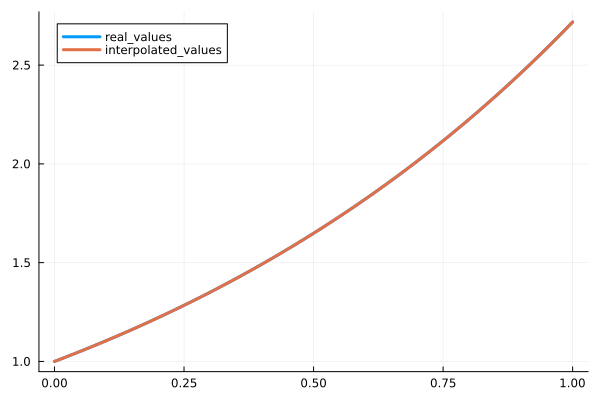
\includegraphics[width=\linewidth]{graphs/zad5.a.5.png}
			\caption{$n = 5$}
		\end{subfigure}
		\begin{subfigure}[b]{\v\linewidth}
			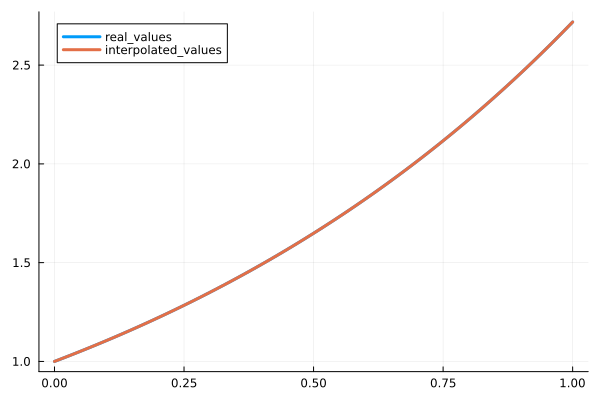
\includegraphics[width=\linewidth]{graphs/zad5.a.10.png}
			\caption{$n = 10$}
		\end{subfigure}
		\begin{subfigure}[b]{\v\linewidth}
			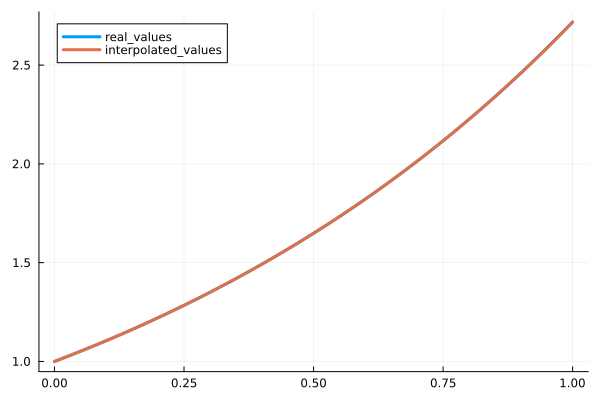
\includegraphics[width=\linewidth]{graphs/zad5.a.15.png}
			\caption{$n = 15$}
		\end{subfigure}
	\\{$f(x) = e^x$ w przedziale $[0;1]$ dla $n = 5,10,15$}
	\end{figure}

	\begin{figure}[H]
	    \centering
		\begin{subfigure}[b]{\v\linewidth}
			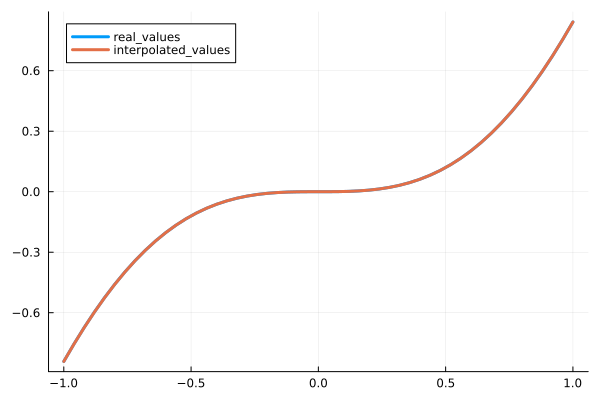
\includegraphics[width=\linewidth]{graphs/zad5.b.5.png}
			\caption{$n = 5$}
		\end{subfigure}
		\begin{subfigure}[b]{\v\linewidth}
			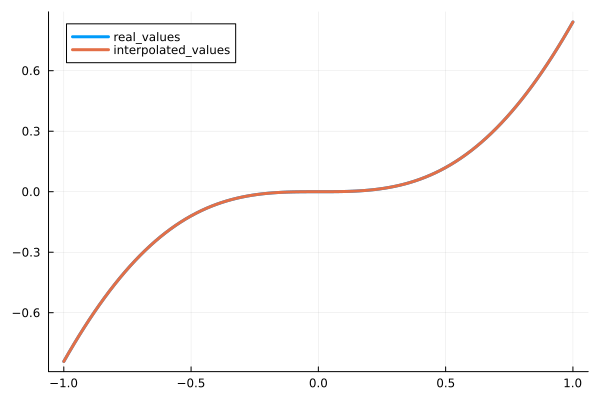
\includegraphics[width=\linewidth]{graphs/zad5.b.10.png}
			\caption{$n = 10$}
		\end{subfigure}
		\begin{subfigure}[b]{\v\linewidth}
			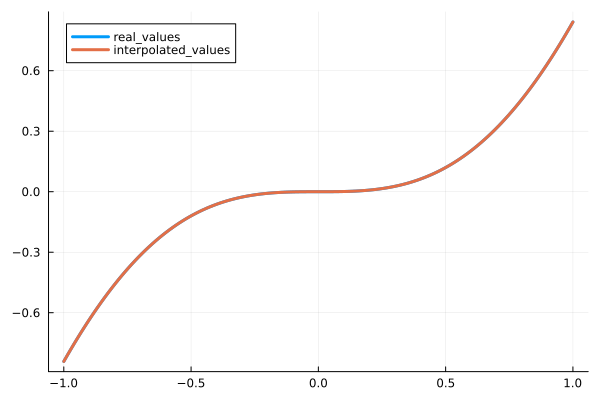
\includegraphics[width=\linewidth]{graphs/zad5.b.15.png}
			\caption{$n = 15$}
		\end{subfigure}
	\\{$f(x) = x^2 \cdot sin x$ w przedziale $[-1;1]$ dla $n = 5,10,15$}
	\end{figure}
\subsection*{Wnioski}

\section*{Zadanie 6}
	Przetestować metodę \texttt{draw\_Nnfx} na kilku zadanych poniżej funkcjach.
\subsection*{Wyniki}
	\begin{figure}[H]
	    \centering
		\begin{subfigure}[b]{\v\linewidth}
			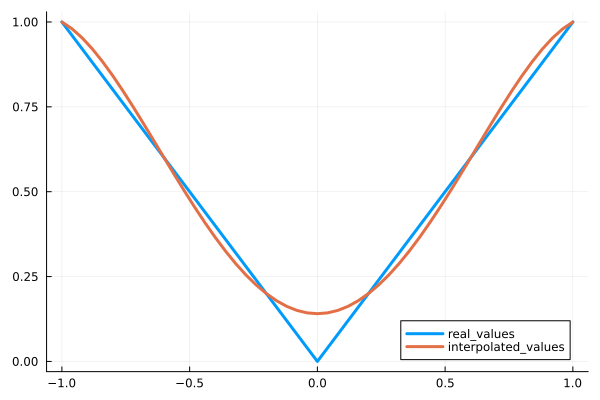
\includegraphics[width=\linewidth]{graphs/zad6.a.5.png}
			\caption{$n = 5$}
		\end{subfigure}
		\begin{subfigure}[b]{\v\linewidth}
			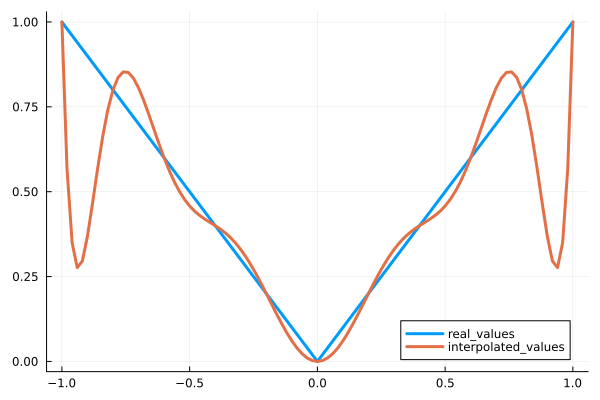
\includegraphics[width=\linewidth]{graphs/zad6.a.10.png}
			\caption{$n = 10$}
		\end{subfigure}
		\begin{subfigure}[b]{\v\linewidth}
			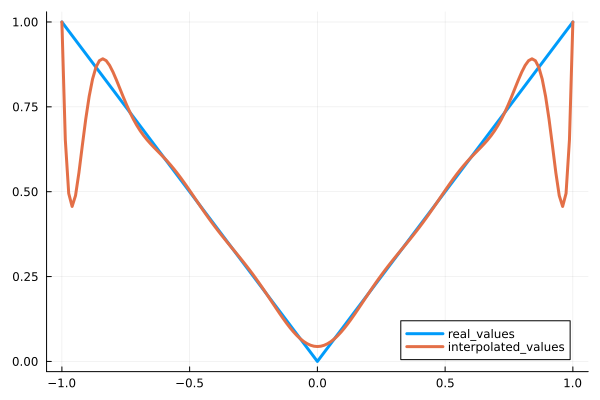
\includegraphics[width=\linewidth]{graphs/zad6.a.15.png}
			\caption{$n = 15$}
		\end{subfigure}
	\\{$f(x) = |x|$ w przedziale $[-1;1]$ dla $n = 5,10,15$}
	\end{figure}

	\begin{figure}[H]
	    \centering
		\begin{subfigure}[b]{\v\linewidth}
			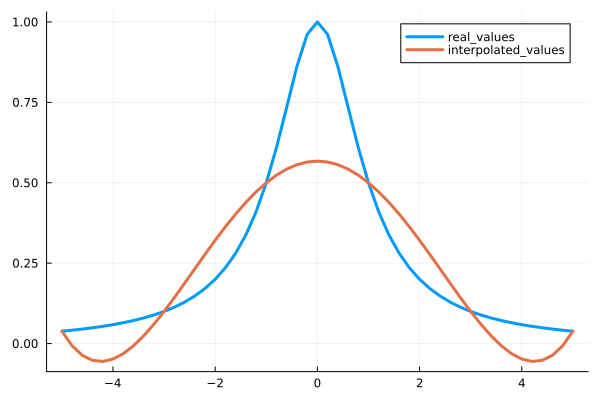
\includegraphics[width=\linewidth]{graphs/zad6.b.5.png}
			\caption{$n = 5$}
		\end{subfigure}
		\begin{subfigure}[b]{\v\linewidth}
			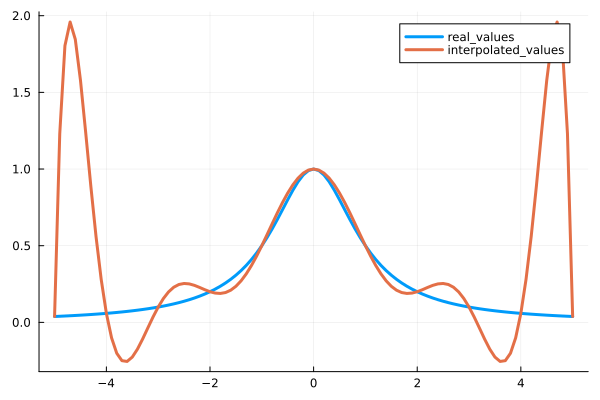
\includegraphics[width=\linewidth]{graphs/zad6.b.10.png}
			\caption{$n = 10$}
		\end{subfigure}
		\begin{subfigure}[b]{\v\linewidth}
			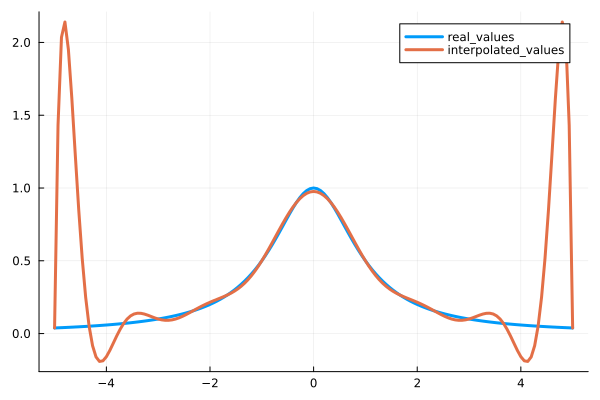
\includegraphics[width=\linewidth]{graphs/zad6.b.15.png}
			\caption{$n = 15$}
		\end{subfigure}
	\\{$f(x) = \frac{1}{1+x^2}$ w przedziale $[-5;5]$ dla $n = 5,10,15$}
	\end{figure}
\subsection*{Wnioski}

\end{document}